%!TEX root =../main-tokyo.tex
% ##################################################################################################################
\chapter{Joinville}
\label{ch:joinville}
\hfill \textbf{Authors:} Davi Guggisberg Bicudo, Gian Ricardo Berkenbrock

% ##################################################################################################################
Joinville \cite{pmj} is a mid-sized industrial city in the south of Brazil with around 550\,000 inhabitants. It has a large workforce, including from its neighboring cities. As it has an intense industrial activity profile, companies work often in three shifts, which cause peculiar traffic patterns. Besides this, it is common to have people with 12-hour routines considering work and higher education. 

The Joinville traffic model was built as an initial step of a project that intends to simulate the entire northeast region of Santa Catarina State, including air traffic, shipping, state highways and neighboring cities. The aim of the project is a wide comprehension of people and freight movement on the region. The urban Joinville model is on its first version now and was produced as a graduation thesis at the Federal University of Santa Catarina (UFSC) \url{http://ufsc.br}, course of Transportation and Logistics Engineering \url{http://transporteslogistica.joinville.ufsc.br}.%
\footnote{The authors would like to thank their sponsors Federal University of Santa Catarina (UFSC) and Urban Sustainable Planning Institute of Joinville (IPPUJ).} 

The scenario population was generated with data from the 2010~Brazilian census combined with demographic information from the city’s travel survey. Travel demand was generated from the same travel survey. Both were designed to fit into the \gls{matsim} using Tutorial classes (with some adaptations).

The network was produced with vector data provided by the local Urban Sustainable Planning Institute of Joinville (IPPUJ) \url{https://ippuj.joinville.sc.gov.br}. The data came as a shapefile with many connectivity problems. We were able to fix them using scripts in Python with the \lstinline|NetworkX| module \cite{networkx}. Transforming was performed from the vector data into a graph, fixing the issues with the help of \gls{qgis} and finally writing as the \gls{matsim} \gls{xml} network format. The facilities were produced from land-use data provided from the city's government.

For now the model runs only with cars. The model used a full sample of the population. From the available data we inferred 135\,652 agents that did their routines by car, the rest were removed of the simulation. Figure~\ref{fig:Joinville_ssMain} shows a screenshot of the Events using \gls{via}.

The Figure~\ref{fig:Joinville_counts} shows the comparison between simulated and count data for 20\,links in the morning peak from 7 to 8\,AM. The count data available for comparison is still sparse which could not provide us with a good measure of success. We know that calibration is needed for the next versions of the model. The good news is that the local authorities are installing over a hundred counting stations throughout the city within the next couple months and a new travel survey will be held this year. 

\createfigure%
{Screenshot of the simulation using \gls{via}}%
{Screenshot of the simulation using \gls{via}}%
{\label{fig:Joinville_ssMain}}%
{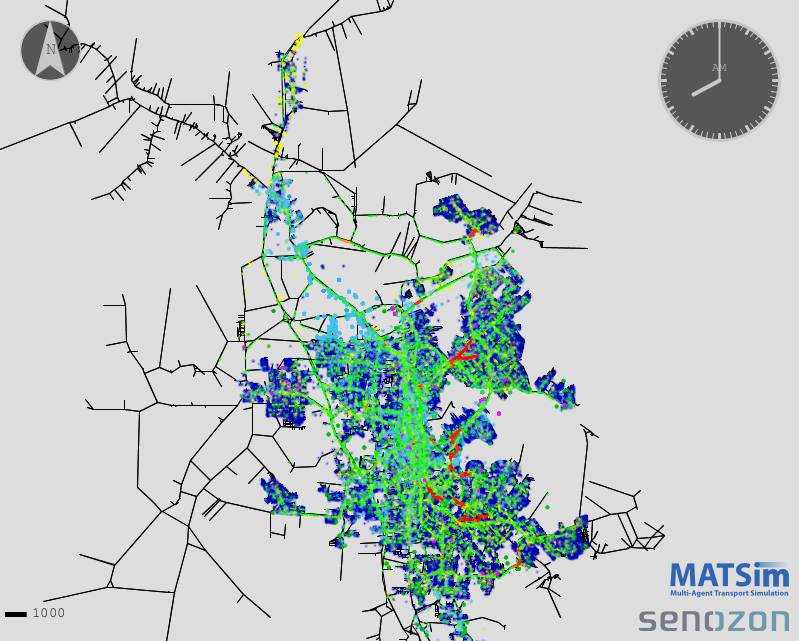
\includegraphics[width=0.7\textwidth, angle=0]{./scenarios/figures/Joinville_ssMain.png}}%
{}

\createfigure%
{Count comparisons for the morning peak at 7-8 AM}%
{Count comparisons for the morning peak at 7-8 AM}%
{\label{fig:Joinville_counts}}%
{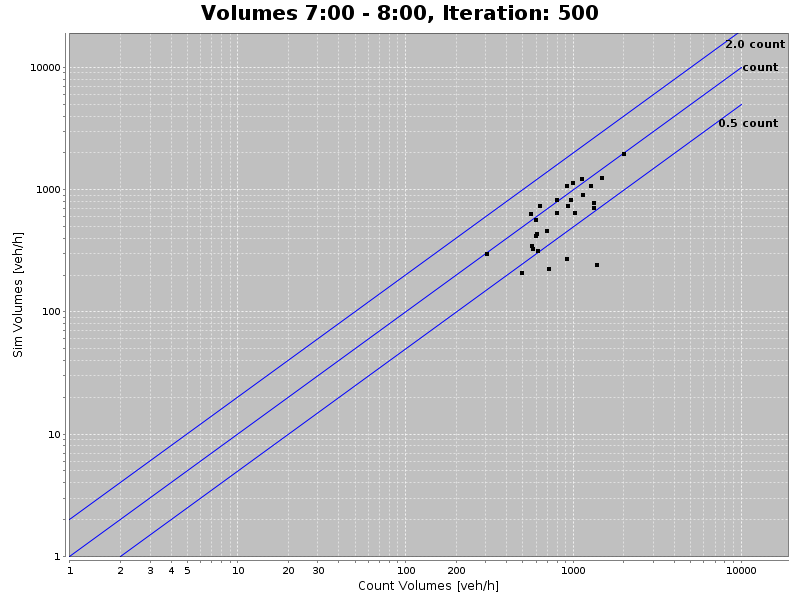
\includegraphics[width=0.7\textwidth, angle=0]{./scenarios/figures/Joinville_LogManha.png}}%
{}

% ##################################################################################################################